%----------------------------------------------------------------------------------------
%	PACKAGES AND OTHER DOCUMENT CONFIGURATIONS
%----------------------------------------------------------------------------------------

\documentclass{article}

\usepackage{fancyhdr} % Required for custom headers
\usepackage{lastpage} % Required to determine the last page for the footer
\usepackage{extramarks} % Required for headers and footers
\usepackage[usenames,dvipsnames]{color} % Required for custom colors
\usepackage{graphicx} % Required to insert images
\usepackage{amsmath}% http://ctan.org/pkg/amsmath
\usepackage{listings} % Required for insertion of code
\usepackage{bm}
%\usepackage{couriernew} % Required for the courier font

\usepackage{enumerate} % Required for enumerating with letters

\usepackage{mathpazo}
\usepackage{avant}
\usepackage{inconsolata}

\newcommand{\tr}{\text{tr}}
\newcommand{\pN}{\mathcal{N}}
\newcommand{\R}{\textsf{R} }
\newcommand{\1}{\mathbf{1}}
\newcommand{\0}{\mathbf{0}}
\newcommand{\x}{\mathbf{x}}
\newcommand{\f}{\mathbf{f}}
\newcommand{\y}{\mathbf{y}}


% \newcommand{\1}{\bm{1}}
% \newcommand{\0}{\bm{0}}
% \newcommand{\x}{\bm{x}}
% \newcommand{\f}{\bm{f}}
% \newcommand{\y}{\bm{y}}

\newcommand{\iid}{\overset{\text{iid}}{\sim}}
\newcommand\independent{\protect\mathpalette{\protect\independenT}{\perp}}
\def\independenT#1#2{\mathrel{\rlap{$#1#2$}\mkern2mu{#1#2}}}

% Margins
\topmargin=-0.45in
\evensidemargin=0in
\oddsidemargin=0in
\textwidth=6.5in
\textheight=9.0in
\headsep=0.25in

\linespread{1.1} % Line spacing

% Set up the header and footer
\pagestyle{fancy}
\lhead{\hmwkAuthorName} % Top left header
\chead{\hmwkClass\ : \hmwkTitle} % Top center head
\rhead{} % Top right header
\lfoot{\lastxmark} % Bottom left footer
\cfoot{} % Bottom center footer
\rfoot{Page\ \thepage\ of\ \protect\pageref{LastPage}} % Bottom right footer
\renewcommand\headrulewidth{0.4pt} % Size of the header rule
\renewcommand\footrulewidth{0.4pt} % Size of the footer rule

\setlength\parindent{0pt} % Removes all indentation from paragraphs

%----------------------------------------------------------------------------------------
%	CODE INCLUSION CONFIGURATION
%----------------------------------------------------------------------------------------

\definecolor{MyDarkGreen}{rgb}{0.0,0.4,0.0} % This is the color used for comments
\lstloadlanguages{R} % Load R syntax for listings, for a list of other languages supported see: ftp://ftp.tex.ac.uk/tex-archive/macros/latex/contrib/listings/listings.pdf
\lstset{language=R, % Use R in this example
        frame=single, % Single frame around code
        basicstyle=\small\ttfamily, % Use small true type font
        keywordstyle=[1]\color{Blue}, % Perl functions bold and blue
        keywordstyle=[2]\color{Purple}, % Perl function arguments purple
        keywordstyle=[3]\color{Blue}\underbar, % Custom functions underlined and blue
        identifierstyle=, % Nothing special about identifiers                                         
        commentstyle=\usefont{T1}{pcr}{m}{sl}\color{MyDarkGreen}\small, % Comments small dark green courier font
        stringstyle=\color{Purple}, % Strings are purple
        showstringspaces=false, % Don't put marks in string spaces
        tabsize=4, % 5 spaces per tab
        %
        % Put standard Perl functions not included in the default language here
        morekeywords={rand},
        %
        % Put Perl function parameters here
        morekeywords=[2]{on, off, interp},
        %
        % Put user defined functions here
        morekeywords=[3]{test},
       	%
        morecomment=[l][\color{Blue}]{...}, % Line continuation (...) like blue comment
        numbers=left, % Line numbers on left
        firstnumber=1, % Line numbers start with line 1
        numberstyle=\tiny\color{Blue}, % Line numbers are blue and small
        stepnumber=5 % Line numbers go in steps of 5
}

% Creates a new command to include a perl script, the first parameter is the filename of the script (without .pl), the second parameter is the caption
\newcommand{\rscript}[2]{
\begin{itemize}
\item[]\lstinputlisting[caption=#2,label=#1]{#1.r}
\end{itemize}
}

%----------------------------------------------------------------------------------------
%	DOCUMENT STRUCTURE COMMANDS
%	Skip this unless you know what you're doing
%----------------------------------------------------------------------------------------

% Header and footer for when a page split occurs within a problem environment
\newcommand{\enterProblemHeader}[1]{
\nobreak\extramarks{#1}{#1 continued on next page\ldots}\nobreak
\nobreak\extramarks{#1 (continued)}{#1 continued on next page\ldots}\nobreak
}

% Header and footer for when a page split occurs between problem environments
\newcommand{\exitProblemHeader}[1]{
\nobreak\extramarks{#1 (continued)}{#1 continued on next page\ldots}\nobreak
\nobreak\extramarks{#1}{}\nobreak
}

\setcounter{secnumdepth}{0} % Removes default section numbers
\newcounter{homeworkProblemCounter} % Creates a counter to keep track of the number of problems

\newcommand{\homeworkProblemName}{}
\newenvironment{homeworkProblem}[1][Problem \arabic{homeworkProblemCounter}]{ % Makes a new environment called homeworkProblem which takes 1 argument (custom name) but the default is "Problem #"
\stepcounter{homeworkProblemCounter} % Increase counter for number of problems
\renewcommand{\homeworkProblemName}{#1} % Assign \homeworkProblemName the name of the problem
\section{\homeworkProblemName} % Make a section in the document with the custom problem count
\enterProblemHeader{\homeworkProblemName} % Header and footer within the environment
}{
\exitProblemHeader{\homeworkProblemName} % Header and footer after the environment
}

\newcommand{\problemAnswer}[1]{ % Defines the problem answer command with the content as the only argument
\noindent\framebox[\columnwidth][c]{\begin{minipage}{0.98\columnwidth}#1\end{minipage}} % Makes the box around the problem answer and puts the content inside
}

\newcommand{\homeworkSectionName}{}
\newenvironment{homeworkSection}[1]{ % New environment for sections within homework problems, takes 1 argument - the name of the section
\renewcommand{\homeworkSectionName}{#1} % Assign \homeworkSectionName to the name of the section from the environment argument
\subsection{\homeworkSectionName} % Make a subsection with the custom name of the subsection
\enterProblemHeader{\homeworkProblemName\ [\homeworkSectionName]} % Header and footer within the environment
}{
\enterProblemHeader{\homeworkProblemName} % Header and footer after the environment
}

%----------------------------------------------------------------------------------------
%	NAME AND CLASS SECTION
%----------------------------------------------------------------------------------------

\newcommand{\hmwkTitle}{Exercises 3 -- Linear smoothing and Gaussian processes} % Assignment title
\newcommand{\hmwkDueDate}{\today} % Due date
\newcommand{\hmwkClass}{SDS\ 383D} % Course/class
\newcommand{\hmwkClassTime}{} % Class/lecture time
\newcommand{\hmwkClassInstructor}{Professor Scott} % Teacher/lecturer
\newcommand{\hmwkAuthorName}{Spencer Woody} % Your name

%----------------------------------------------------------------------------------------
%	TITLE PAGE
%----------------------------------------------------------------------------------------

\title{
\vspace{2in}
\textmd{\textbf{\hmwkClass:\ \hmwkTitle}}\\
\normalsize\vspace{0.1in}\small{\hmwkDueDate}\\
\vspace{0.1in}\large{\textit{\hmwkClassInstructor\ }}
\vspace{3in}
}

\author{\textbf{\hmwkAuthorName}}
\date{} % Insert date here if you want it to appear below your name

%----------------------------------------------------------------------------------------

\begin{document}

\maketitle

\newpage

%----------------------------------------------------------------------------------------
%	PROBLEM 1
%----------------------------------------------------------------------------------------

% To have just one problem per page, simply put a \clearpage after each problem

\begin{homeworkProblem}

\large
\textbf{Basic Concepts}
\normalsize


\begin{enumerate}[(A)]
	\item % A
	%
	%
	%
	%
	%
	%
	%
\end{enumerate}




\end{homeworkProblem}

%----------------------------------------------------------------------------------------
%	PROBLEM 2
%----------------------------------------------------------------------------------------

% To have just one problem per page, simply put a \clearpage after each problem

\pagebreak

\begin{homeworkProblem}

\large
\textbf{Curve fitting by linear smoothing}
\normalsize

In this problem, consider a general nonlinear regression with one predictor and one response, $y_i = f(x_i) + \epsilon_i$, where $\epsilon_i$ are mean-zero random variables.

\begin{enumerate}[(A)]
	\item % A
	%
	%
	%
	For now, consider a linear regression on a response $y_i$ with one predictor $x_i$, and both $y_i$ and $x_i$ have had their means subtracted, so the $y_i = \beta x_i + \epsilon_i$. Define $S_x := \sum_{i=1}^n x_i^2.$ The least squares estimate for the coefficient, from Exercises 1, is 
	%
	%
	%
	\begin{align*}
		\hat{\beta} &= (X^TX)^{-1}X^Ty \\
			 		&= (x^Tx)^{-1}x^T y \\
					&= \frac{\sum_{i=1}^n x_i \cdot y_i}{\sum_{i=1}^n x_i^2} \\
					&= \frac{\sum_{i=1}^n x_i \cdot y_i}{S_x} \\ 
					&= \sum_{i=1}^n \frac{x_i}{S_x} \cdot y_i.
	\end{align*}
	%
	%
	%
	So now our prediction $y^\star | x^\star$ is, 
	%
	%
	%
	\begin{align*}
		\hat{y}^\star &= \hat{f}(x^\star) \\
		&= \hat{\beta}x^\star \\
		&= \left( \sum_{i=1}^n \frac{x_i}{S_x} \cdot y_i \right) \cdot x^\star \\
		&= \sum_{i=1}^n \left( \frac{x_i}{S_x} \cdot x^\star \right) \cdot y_i,
	\end{align*}
	%
	%
	%
	which we recognize as being in the form of the general \emph{linear smoother}
	%
	%
	%
	\begin{align*}
		\hat{f}\left( x^\star \right) &= \sum_{i=1}^n w(x_i, x^\star) \cdot y_i
	\end{align*}
	%
	%
	%
	for some weight function $w(x_i, x^\star)$. In particular, the weight function for linear regression gives weight to each $y_i$ proportional to the value of $x_i$. Contrast this with the $k$-nearest neighbors smoothing weight function,
	%
	%
	%
	\begin{align*}
		w_K(x_i, x^\star) &= \begin{cases}
			1/K & \text{if } x_i \text{ is one of the K closest sample points to } x^\star \\
			0 & \text{otherwise} 
		\end{cases},
	\end{align*}
	%
	%
	%
	which gives \emph{equal} weight to $y_i$s but \emph{only} to the $k$-nearest neighbors of $x^\star$.
	%
	%
	%
	\item % B
	%
	%
	%
	Now we have the very general weight function
	%
	%
	%
	\begin{align*}
		w(x_i, x^\star) &= \frac{1}{h} \cdot K\left( \frac{x_i - x^\star}{h}, \right)
	\end{align*}
	%
	%
	%
	where $K(\bullet)$ is some kernel function. The script \texttt{myfuns03.R} in the appendix shows an \textsf{R} function for linear smoothing, as well functions for the uniform and Gaussian kernels. Figure \ref{fig:firstexample} shows an example of smoothing with a bandwidth of 0.75 for a cubic function $f(x)$ with iid residuals from the $\pN(0, 15^2)$ distribution. 
	%
	%
	%
	\begin{figure}[htp!]
		\centering
			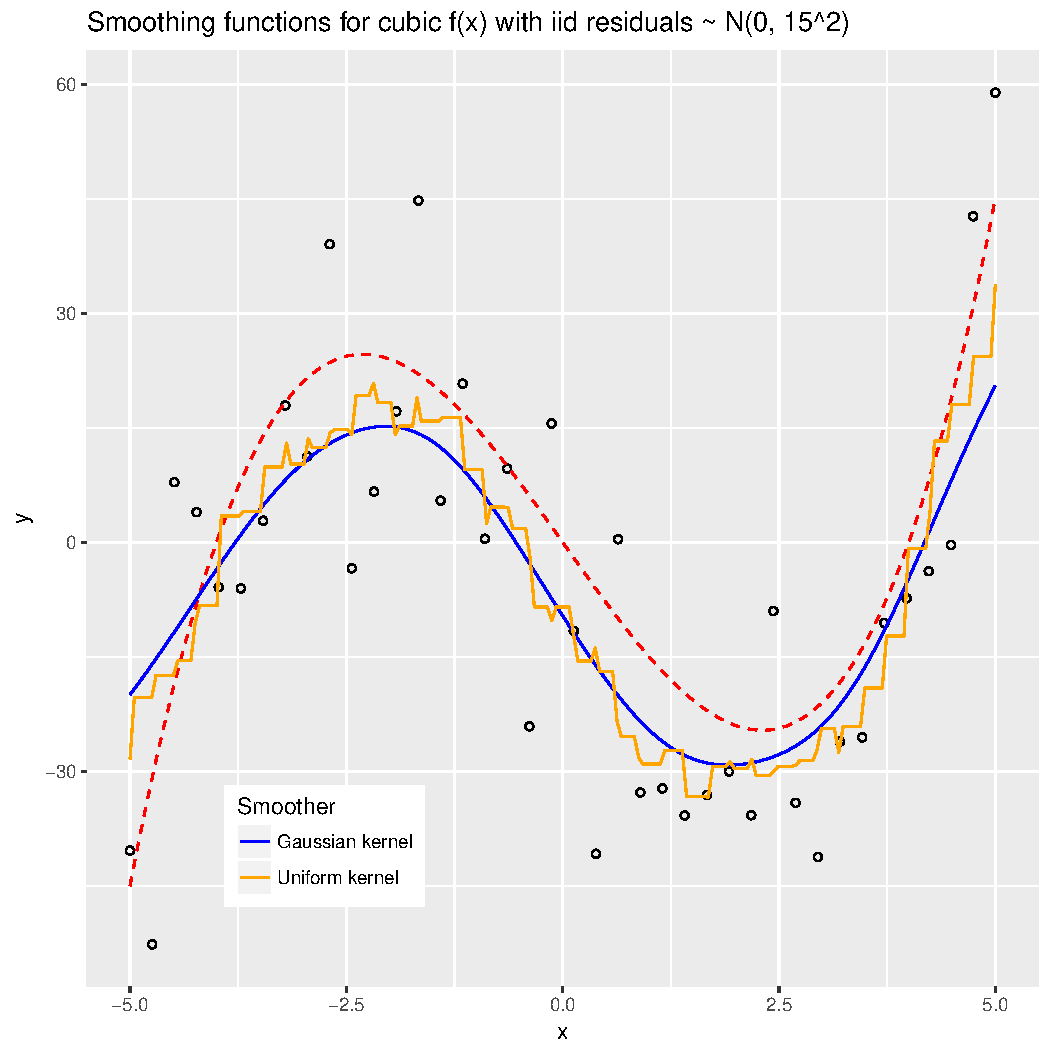
\includegraphics[scale=0.5]{firstexample.pdf}
		\caption{Uniform and Gaussian kernel smoothing for $y=f(x) + e$, $f(x) = x(x-4)(x+4)$, $h=0.75$}
		\label{fig:firstexample}
	\end{figure}
	%
	%
	%
\end{enumerate}

\end{homeworkProblem}

%----------------------------------------------------------------------------------------
%	PROBLEM 3
%----------------------------------------------------------------------------------------

\pagebreak

% To have just one problem per page, simply put a \clearpage after each problem

\begin{homeworkProblem}

\large
\textbf{Cross validation}
\normalsize


\begin{enumerate}[(A)]
	\item % A
	%
	%
	%
	See attached \R code for a script to return prediction error estimates for smoothing given a specified choice of bandwidth, $h$.
	%
	%
	%
	\item
	%
	%
	%
	For this exercise, I produced 500 data points on the $x$-space $[0, 1]$ from a sine function $f(x)$ with a given period and set the amplitude, and added Gaussian noise with a given standard deviation. Then I used 5-fold cross validation to select the optimal bandwidth for that given period and standard deviation of noise term. Figure \ref{fig:heatmap} shows the optimal bandwidths for period ranging from 0.1 to 1, and standard deviation ranging from 0.001 to 0.5, and Figure \ref{fig:2x2} shows four example The highest bandwidths are chosen for functions with high ``wigglyness'' and high noise, and the smallest bandwidths are chosen for functions with low ``wigglyness'' and low noise. This makes sense. As the frequency increases (i.e., period decreases) then we need a tighter bandwidth because the value of the function is fluctuating at a greater rate. As noise increases, we need a greater bandwidth to smooth out the noise. Furthermore, we can see that in all cases we recover the underlying function pretty well.
	%
	%
	%
	\begin{figure}[htp!]
		\centering
			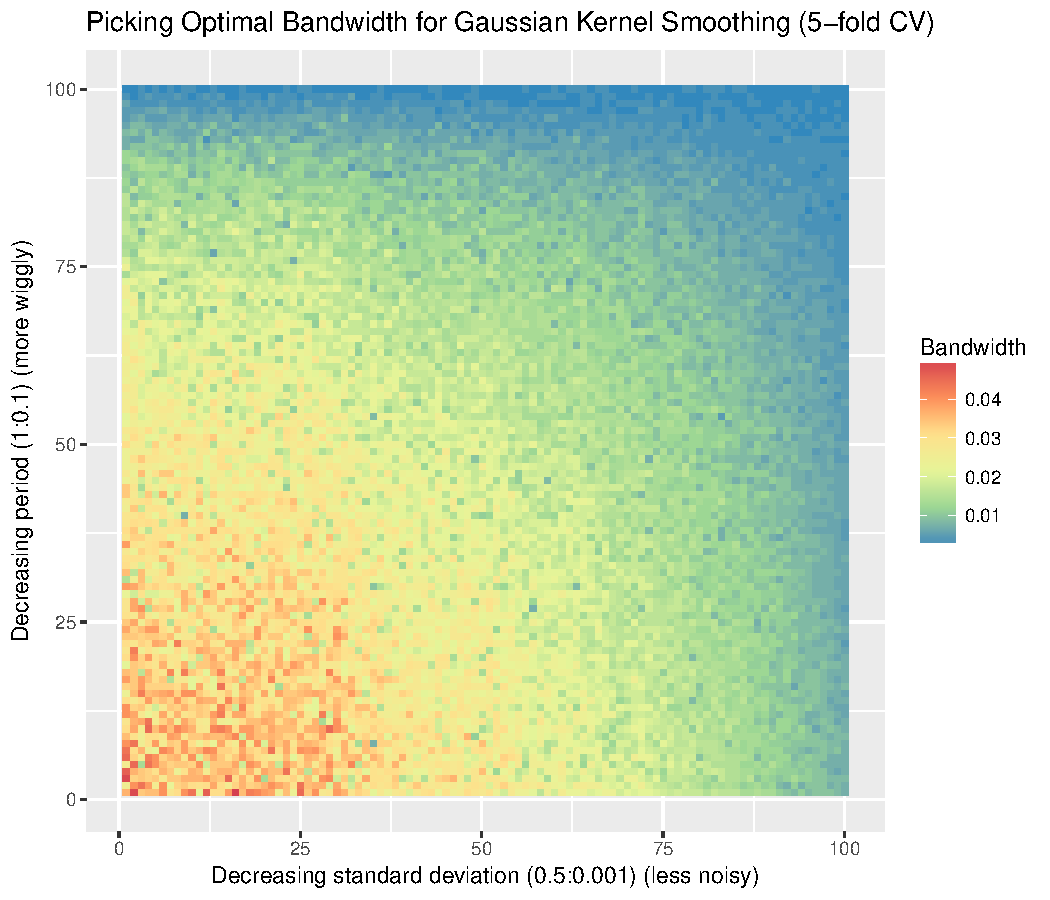
\includegraphics[scale=0.5]{img/opth.pdf}
		\caption{Optimal bandwidths for varying periods and standard deviations}
		\label{fig:heatmap}
	\end{figure}
	%
	%
	%
	\begin{figure}[htp!]
		\centering
			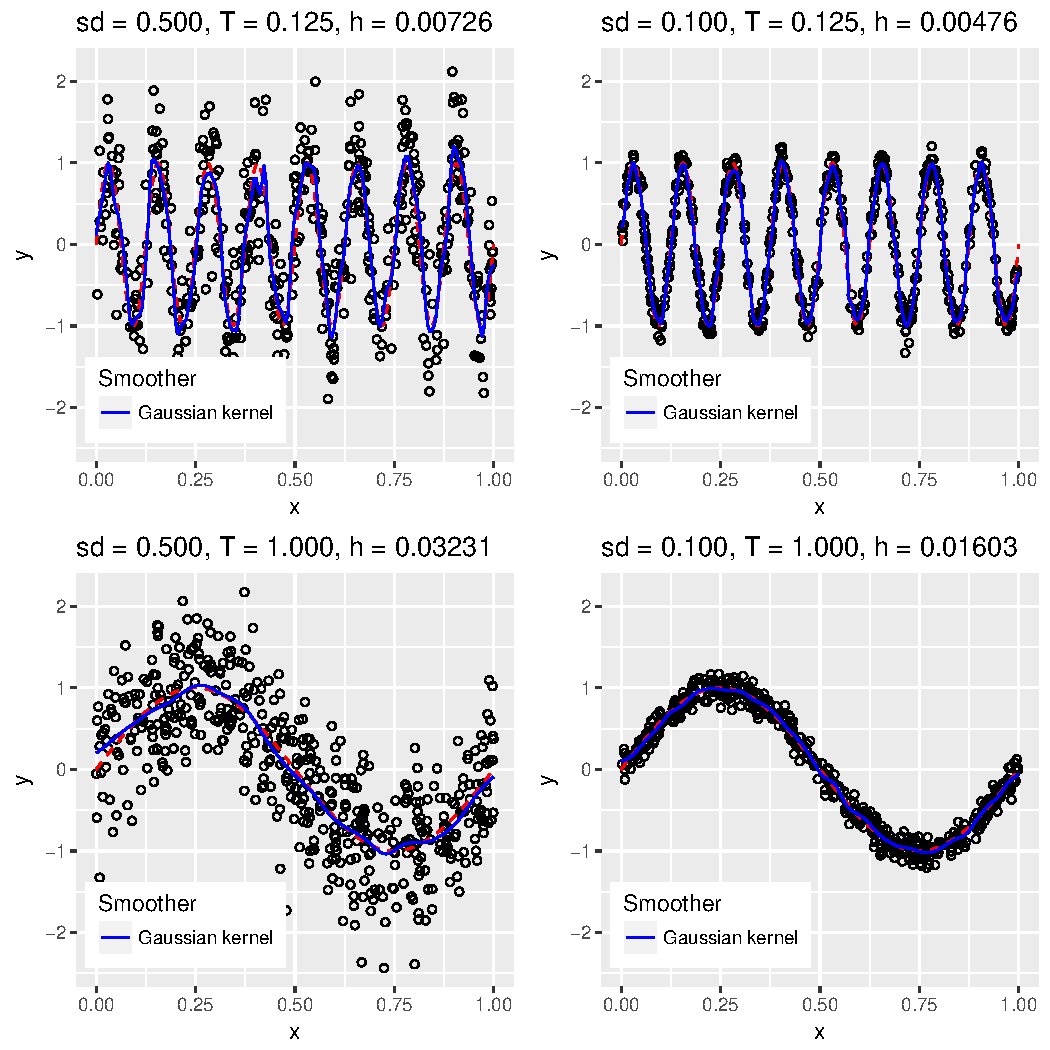
\includegraphics[scale=0.5]{img/2x2.pdf}
		\caption{$2\times2$ example with fitted curves}
		\label{fig:2x2}
	\end{figure}
	%
	%
	%
	\item % LOOCV
	%
	%
	%
	I'll get around to this eventually\ldots.
	%
	%
	%
\end{enumerate}

\end{homeworkProblem}

%----------------------------------------------------------------------------------------
%	PROBLEM 4
%----------------------------------------------------------------------------------------

\pagebreak

\begin{homeworkProblem}

\large
\textbf{Local polynomial regression}
\normalsize


\begin{enumerate}[(A)]
	\item % A
	%
	%
	%
	Define
	%
	%
	%
	\begin{align*}
		g_x(u; a) &= a_0 + \sum_{k=1}^D a_k (u - x)^k \\
		&= \begin{cases}
			\sum_{j=0}^{D+1} a_j (u - x)^j &\;\text{ if } u \neq x \\
			a_0 &\;\text{ if } u = x
		\end{cases}.
	\end{align*}
	%
	%
	%
	The coefficients of $a$ for the local polynomial regression with dimension $D$ will come from the weighted least squares problem 
	%
	%
	%
	\begin{align}
		\hat{a} &= \arg \min_{a \in \mathcal{R}^{D+1}} \sum_{i=1}^n w_i \left[y_i - g_x(x_i, a) \right]^2
	\end{align}
	%
	%
	%
	Furthermore, define the matrix $R_x$ whose $(i, j)$ element is $(x_i - x)^2$. Then the estimate $\hat{f}(x)$ will be $R_x \hat{a}$. The solution of $\hat{a}$ may be found with 
	%
	%
	%
	\begin{align*}
		\hat{a} &= \arg \min_{a \in \mathcal{R}^{D+1}} (y - R_x a)^T W (y - R_x a) \\
		&= (R_x^T W R_x)^{-1}R_x^TWy
	\end{align*}
	%
	%
	%
	where $W = \text{diag}(w_1, \ldots, w_n)$ is a diagonal matrix of weights from some kernel, $$w_i = \frac{1}{h}K\left( \frac{x_i - x}{h}\right)$$ and this solution is found following the same argument to find the WLS estimate of linear regression from Exercises 1.
	%
	%
	%
	\item % B
	%
	%
	%
	Define the matrix $B_x = (R_x^T W R_x)^{-1}R_x^TW$. The estimate of $f$ at a point $x^\star$ is $\hat{f}(x) = \hat{a}_0$, the first element of the vector $\hat{a}$ whose form is derived above. Since our estimate is in the form of a linear smoother, this can also be written as $\hat{f}(x) = \frac{b_x^T y}{\sum_{i=1}^n b_{x, i}}$ if we take $b^T$ to be the first row of $B$. In the special case of the local linear smoother ($D=1$), the matrix $R_x$ has dimension $n \times 2$ and can be written as 
	%
	%
	%
	\begin{align*}
		R_x &= \begin{bmatrix}
			1 & x_1 - x \\
			\vdots & \vdots \\
			1 & x_n - x
		\end{bmatrix}.
	\end{align*}
	%
	%
	%
	\begin{align*}
		R_x^T &= \begin{bmatrix}
			1 & \ldots & 1 \\
			x_1 - x & \ldots & x_n - x
		\end{bmatrix}
	\end{align*}
	%
	%
	%
	\begin{align*}
		W &= \begin{bmatrix}
    w_{1} &  & \mathcal{O}\\
    & \ddots & \\
    \mathcal{O} & & w_{n}
  \end{bmatrix}
	\end{align*}
	%
	%
	%
	\begin{align*}
		R_x^T W R_x &= \begin{bmatrix}
			\sum_{i=1}^n w_i & \sum_{i=1}^n w_i (x_i - x)  \\
			\sum_{i=1}^n w_i (x_i - x) & \sum_{i=1}^n w_i(x_i - x)^2
		\end{bmatrix} ^{-1}
	\end{align*}
	%
	%
	%
	\begin{align*}
		R_x^T W &= \begin{bmatrix}
			w_1 &\ldots & w_n \\
			w_1(x_1 - x) &\ldots & w_n(x_n - x)
		\end{bmatrix}
	\end{align*}
	%
	%
	%
	Furthermore, define the term $$ s_j(x) = \sum_{i=1}^n w_i (x_i - x)^j. $$ Now we can find the exact form of $B$ up to a proportionality constant, 
	%
	%
	%
	\begin{align*}
		B &= (R_x^T W R_x)^{-1}R_x^TW \\
		&= \left( \begin{bmatrix}
			1 & \ldots & 1 \\
			x_1 - x & \ldots & x_n - x
		\end{bmatrix} \begin{bmatrix}
    w_{1} &  & \mathcal{O}\\
    & \ddots & \\
    \mathcal{O} & & w_{n}
  \end{bmatrix} \begin{bmatrix}
			1 & x_1 - x \\
			\vdots & \vdots \\
			1 & x_n - x
		\end{bmatrix} \right)^{-1} \begin{bmatrix}
			1 & \ldots & 1 \\
			x_1 - x & \ldots & x_n - x
		\end{bmatrix} \begin{bmatrix}
    w_{1} &  & \mathcal{O}\\
    & \ddots & \\
    \mathcal{O} & & w_{n}
  \end{bmatrix} \\
  &= \begin{bmatrix}
			\sum_{i=1}^n w_i & \sum_{i=1}^n w_i (x_i - x)  \\
			\sum_{i=1}^n w_i (x_i - x) & \sum_{i=1}^n w_i(x_i - x)^2
		\end{bmatrix} ^{-1} \begin{bmatrix}
			w_1 &\ldots & w_n \\
			w_1(x_1 - x) &\ldots & w_n(x_n - x)
		\end{bmatrix} \\
		&= \begin{bmatrix}
			\sum_{i=1}^n w_i & s_1(x)  \\
			s_1(x) & s_2(x)
		\end{bmatrix} ^{-1} \begin{bmatrix}
			w_1 &\ldots & w_n \\
			w_1(x_1 - x) &\ldots & w_n(x_n - x)
		\end{bmatrix} \\
		&\propto  \begin{bmatrix}
			s_2(x) & -s_1(x)  \\
			-s_1(x) & \sum_{i=1}^n w_i
		\end{bmatrix} \begin{bmatrix}
			w_1 &\ldots & w_n \\
			w_1(x_1 - x) &\ldots & w_n(x_n - x)
		\end{bmatrix} \\
		&= \begin{bmatrix}
			w_1 ( s_2(x) - (x_1 - x) s_1(x) ) &\ldots & w_n \left( s_2(x) - (x_n - x) s_1(x) \right) \\
			w_1 ( (x_1 - x)\sum_{i=1}^n w_i -s_1(x)) & \ldots &w_n ( (x_n - x)\sum_{i=1}^n w_i -s_1(x))
		\end{bmatrix}.
	\end{align*}
	%
	%
	%
	From this we conclude that $\hat{f}(x)$ is a linear smoother with a weight on each $y_i$ proportional to $b_{x,i} = w_i ( s_2(x) - (x_i - x) s_1(x) ).$
	%
	%
	%
	\item % C
	%
	%
	%
	%
	%
	%
	%
	\item % D
	%
	%
	%
	With $H$ a smoothing matrix (or ``hat matrix''), let $r = y - Hy$ be the vector of residuals. If the random vector $x$ with mean vector $\mu$ and covariance matrix $\Sigma$, then $E(x^TQx) = \text{tr}(Q\Sigma) + \mu^T Q \mu$. By assumption, $E(\mathbf{y}) = f(\mathbf{x})$ and $\text{cov}(\mathbf{y}) = \sigma^2 I$ Then, 
	%
	%
	%
	\begin{align*}
		E \left( \| r^2 \|_2^2 \right) &= E \left( (\y - H\y)^T(\y-H\y) \right) \\
		&= E \left( \y^T \y - 2\y^T H \y + \y^T H^T H \y \right) \\
		&= E\left(\y^T \y  \right) - 2 E \left( \y^T H \y \right) + E \left( \y^T H^T H \y \right) \\
		&= \left( \tr\left[ I\sigma^2 I \right] + f(\x)^T f(\x) \right) - 2 \left( \tr\left[ H^T\sigma^2 I \right] + f(\x)^T H^T f(\x) \right) + \left( \tr \left[ H^T H \sigma^2 I \right] + f(\x)^T H^T H f(\x)\right) \\
		&= \left( n\sigma^2 + f(\x)^T f(\x) \right) - 2 \left( \sigma^2 \tr[H] + f(\x)^T H^T f(\x) \right) + \left( \sigma^2 \tr[H^TH] + f(\x)^T H^T H f(\x)\right) \\
		&= \left(n - \tr[H] + \tr [H^T H] \right) \sigma^2 + \left( f(\x)^T f(\x) - 2 f(\x)^T H^T f(\x) + f(\x)^T H^T H f(\x) \right) \\
		&= \left(n - \tr[H] + \tr [H^T H] \right) \sigma^2 + \left( f(\x) - Hf(\x) \right)^T \left( f(\x) - Hf(\x) \right),
	\end{align*}
	%
	%
	%
	so the estimator $$\hat{\sigma}^2 = \frac{\| r^2 \|_2^2}{n - \tr[H] + \tr [H^T H]}$$ will be nearly unbiased in $\sigma^2$ when $f(\x) \approx H f(\x)$.
	%
	%
	%
	\item % E
	%
	%
	%
	See attached \R code for implementation of the local polynomial regression, along with leave-one-out cross validation.
	%
	%
	%
	\item % F
	%
	%
	%
	Fitting this model with $D=1$, the assumption of homoscedasticity (constance variance of residuals) is not met. The residuals fan out towards the lower end of the range for temperature. Taking a logarithmic transform of the response variable, daily gas bill, makes the residuals more uniform, although there are still several outliers in the residuals, now towards the higher ejnd of the range for temperature. See figures below.
	%
	%
	%
	\begin{figure}[htp!]
		\centering
			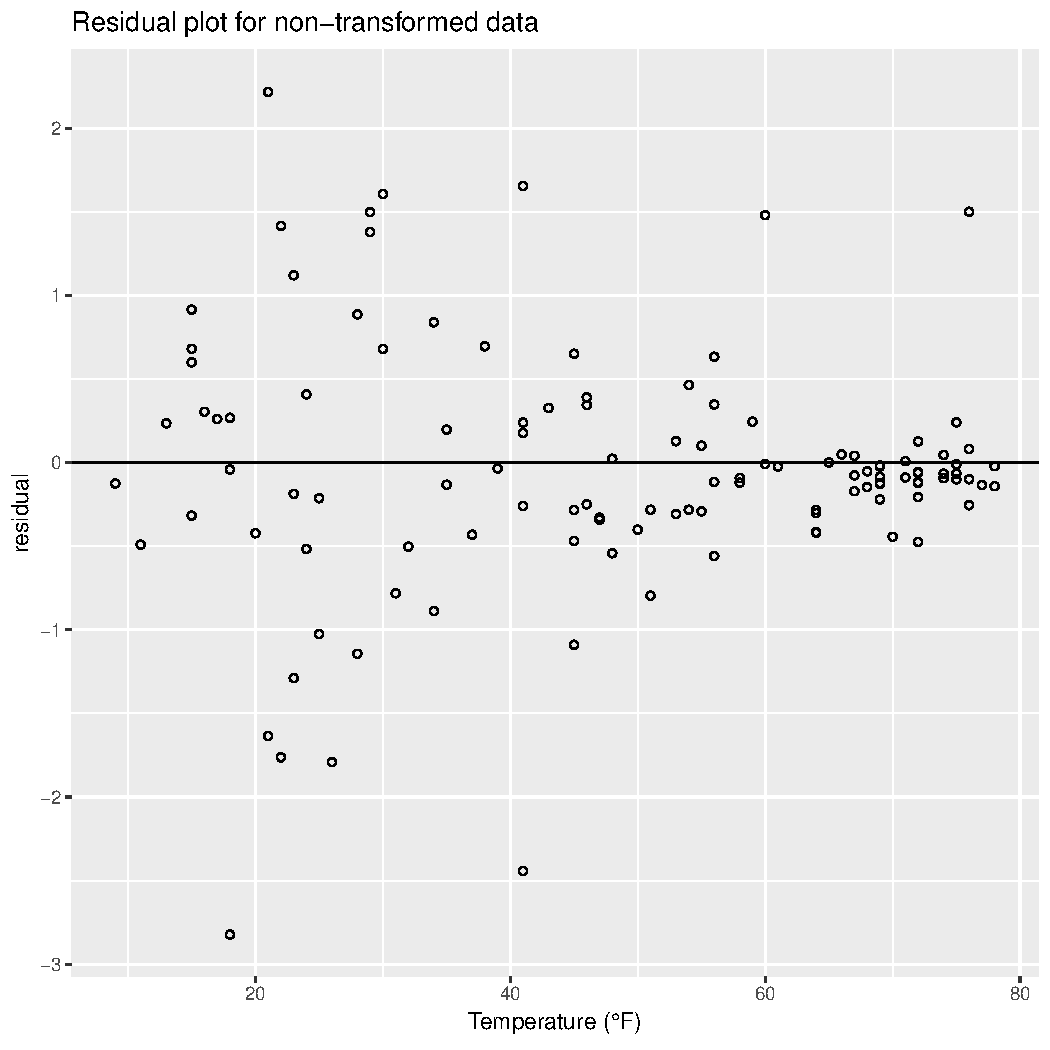
\includegraphics[scale=0.45]{img/resplot1.pdf}
			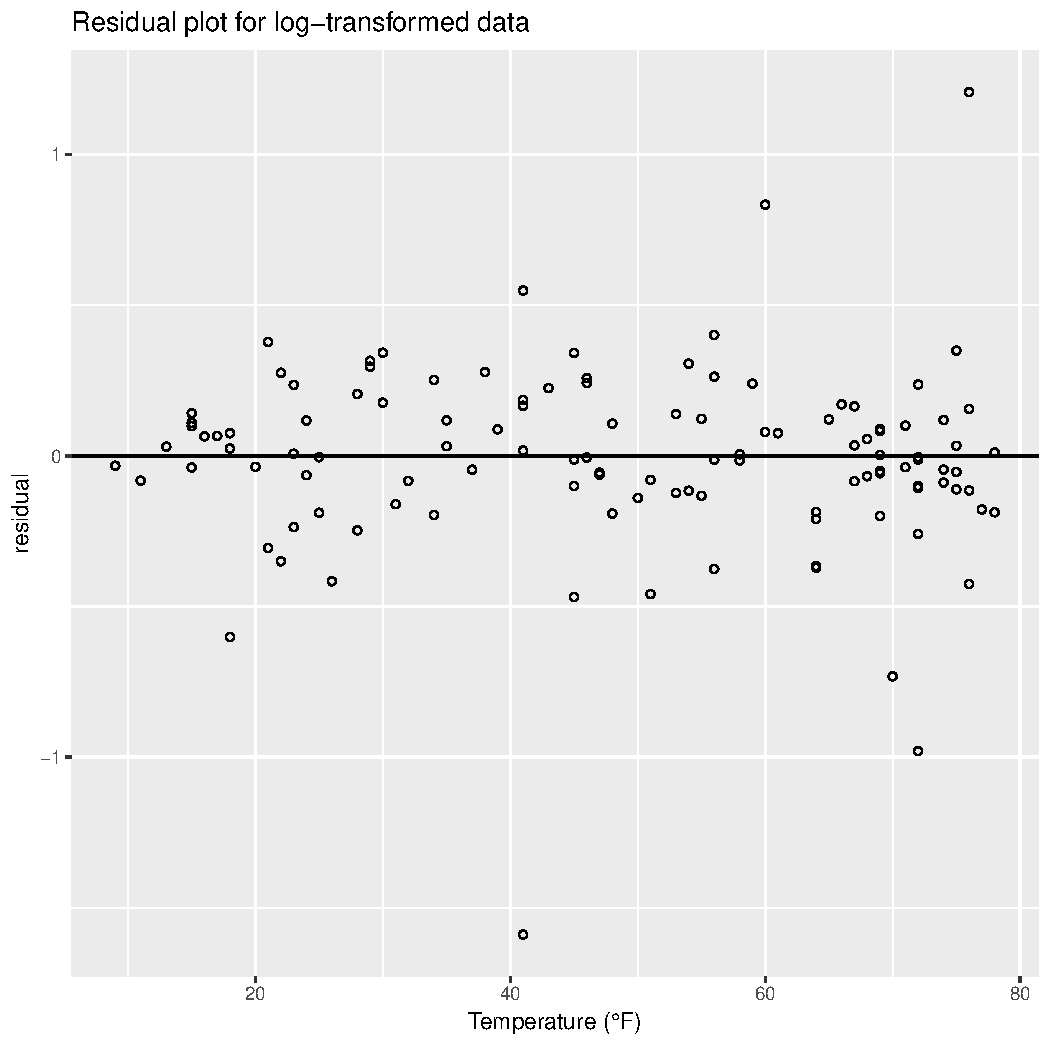
\includegraphics[scale=0.45]{img/resplot2.pdf}
		\caption{Residual plots for models fitted with non-transformed (left) and log-transformed (right) response variables}
	\end{figure}
	%
	%
	%
	\item % G
	%
	%
	%
	The figure below shows the fitted model with 95\% confidence bands (found with $\hat{y} \pm 1.96 \hat{\sigma}$) and overlaid scatterplot of the data. The optimal bandwidth $h = 5.4168$ was chosen with leave-one-out cross validation. The fit is pretty good, with $R^2 = 0.88$, but there are four observations which fall outside the confidence band.
	%
	%
	%
	\begin{figure}[htp!]
		\centering
			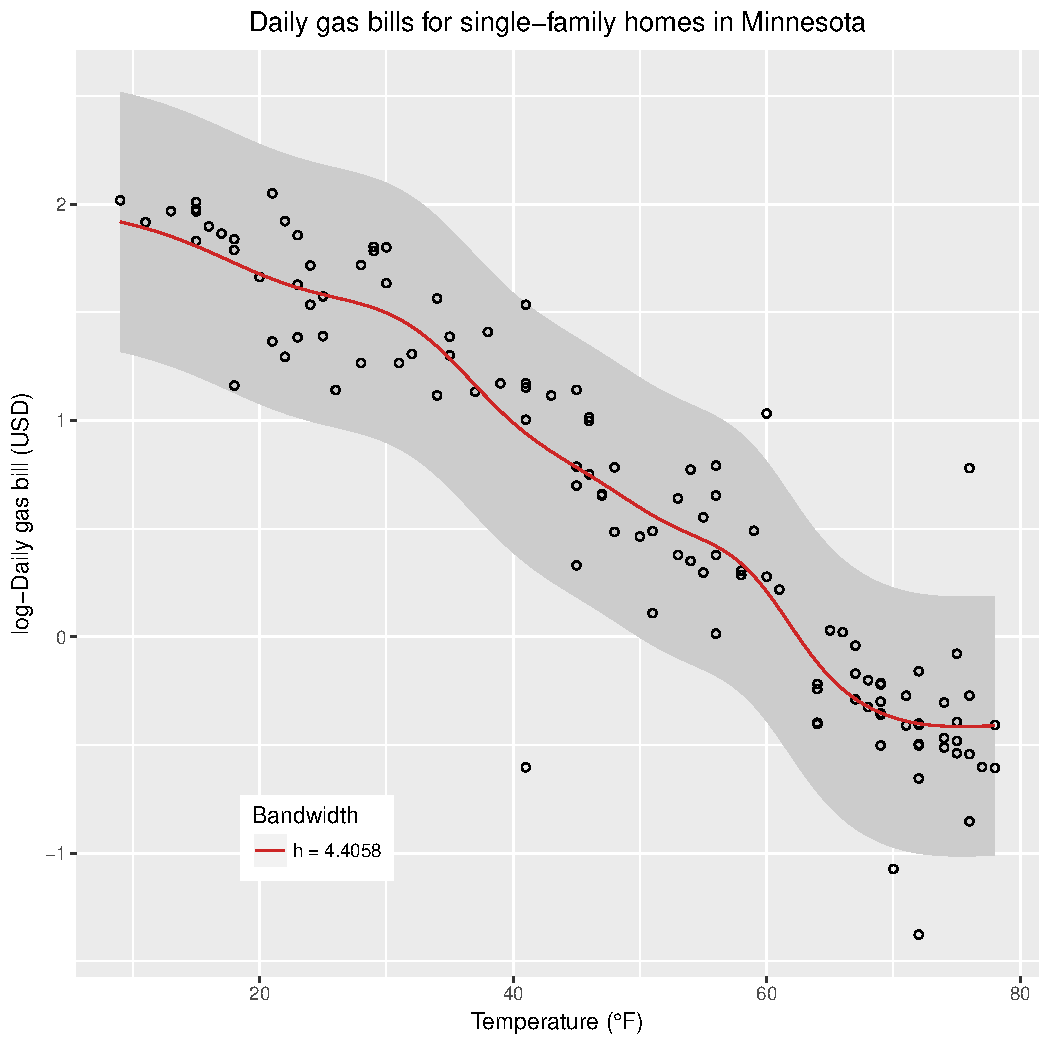
\includegraphics[scale=0.75]{img/tempplot.pdf}
		\caption{Local linear regression for Minnesota gas bill data}
	\end{figure}
	%
	%
	%
\end{enumerate}

\end{homeworkProblem}

%----------------------------------------------------------------------------------------
%	PROBLEM 5
%----------------------------------------------------------------------------------------

\pagebreak

% To have just one problem per page, simply put a \clearpage after each problem

\begin{homeworkProblem}

\large
\textbf{Gaussian processes}
\normalsize


\begin{enumerate}[(A)]
	\item % A
	%
	%
	%
	Examples...
	%
	%
	%
	\item % B
	%
	%
	%
	Suppose that we have a sequence coming from a Gaussian process, $[x_1, x_2, \ldots, x_N, x^\star]^T \sim f \sim \text{GP}(m, C)$ for some mean function $m$ and covariance function $C$. We want to find the distribution of $x^\star$ conditional on the observations $\x = [x_1, x_2, \ldots, x_N]^T$. First, define the three matrices, 
	%
	%
	%
	\begin{align*}
		C &= \begin{bmatrix}
			C(x_1, x_1) & C(x_1, x_2) & \ldots & C(x_1, x_N) \\
			C(x_2, x_1) & C(x_2, x_2) & \ldots & C(x_2, x_N) \\
			\vdots & \vdots & \ddots & \vdots \\
			C(x_N, x_1) & C(x_N, x_2) & \ldots & C(x_N, x_N)
		\end{bmatrix} \\
		C_\star &= \begin{bmatrix}
			C(x^\star, x_1)  & C(x^\star, x_2) & \ldots & C(x^\star, x_N)
		\end{bmatrix} \\
		C_{\star \star} &= \begin{bmatrix}
			C(x^\star, x^\star)
		\end{bmatrix}.
	\end{align*}
	%
	%
	%
	The joint distribution may be written as
	%
	%
	%
	\begin{align*}
		\begin{bmatrix}
			 \x \\
			 x^\star
		\end{bmatrix} &\sim \pN \left(  \begin{bmatrix}
			m(x^\star) \\
			m(\x)
		\end{bmatrix}  , \begin{bmatrix}
			C & C_\star^T \\
			C_\star & C_{\star \star}
		\end{bmatrix} \right).
	\end{align*}
	%
	%
	%
	In Exercises 1, we showed how to derive the conditional distribution from a multivariate normal distribution. Here, we can see that 
	%
	%
	%
	\begin{align*}
		x^\star | \x \sim \pN \left( m(x^\star) + C_\star C^{-1}(\x - m(\x)), C_{\star \star} - C_\star C^{-1} C_\star^T \right).
	\end{align*}
	%
	%
	%
	\item % C
	%
	%
	%
	\end{enumerate}

\end{homeworkProblem}


%----------------------------------------------------------------------------------------
%	PROBLEM 6
%----------------------------------------------------------------------------------------

\pagebreak



% To have just one problem per page, simply put a \clearpage after each problem

\begin{homeworkProblem}

\large
\textbf{In nonparametric regression and spacial smoothing}
\normalsize

	We have the likelihood $y | \theta \sim \pN (R\theta, \Sigma)$ and the prior distribution $\theta \sim \pN(m, V)$. Let $\Omega = \Sigma^{-1}$ and $W = V^{-1}$. We can expand out the respective PDFs of these distributions up to a proportionality constant,
	%
	%
	%
	\begin{align*}
		p(y|\theta) &\propto \exp \left[ -\frac{1}{2} (y-R\theta)^T \Omega (y - R\theta) \right] \\
		&= \exp \left[ -\frac{1}{2} (R\theta - y)^T \Omega (R\theta - y) \right] \\
		&= \exp \left[ -\frac{1}{2} (\theta^T R^T \Omega R \theta - 2y^T\Omega R\theta + y^T\Omega y) \right] \\
		p(\theta)&\propto \exp \left[ -\frac{1}{2} (\theta - m)^TW(\theta-m)\right] \\
		&= \exp \left[ -\frac{1}{2} (\theta^TW\theta - 2m^TW\theta + m^TWm) \right]
	\end{align*}
	%
	%
	%
	Then, by dropping proportionality terms not containing $\theta$ and completing the square, the posterior of $\theta$ is 
	%
	%
	%
	\begin{align*}
		p(\theta | y) &\propto p(y|\theta) p(\theta) \\
		&\propto \exp \left[ -\frac{1}{2} (\theta^T [W + R^T\Omega R] \theta - 2[m^TW + y^T\Omega R] \theta)\right] \\
		&\propto \exp \left[ -\frac{1}{2}(\theta - [W + R^T \Omega R]^{-1}[Wm + R^T\Omega y])^T(W + R^T\Omega R) (\theta - [W + R^T \Omega R]^{-1}[Wm + R^T\Omega y]) \right].
	\end{align*}
	%
	%
	%
	Thus we can see that the posterior distribution is $\theta | y \sim \pN(m', (W')^{-1})$, where
	%
	%
	%
	\begin{align*}
		m' &= (W')^{-1}(Wm + R^T\Omega y) \\
		W' &= W + R^T\Omega R
	\end{align*}
	%
	%
	%


\begin{enumerate}[(A)]
	\item % A
	%
	%
	%
	We observe data $y_i = f(x_i) + \epsilon_i$, where $\epsilon \iid \pN(0, \sigma^2)$ and there is some unknown function $f$. In this problem, we assume $\sigma$ is known. Now we put a mean-zero Gaussian process prior distribution on $f \sim \text{GP}(0, C(\bullet))$ for some covariance function $C(\bullet)$. Let $\x = [x_1, x_2, \ldots, x_N]^T$ denote the previous observed $x$ points. Further, define the random vector $\f = [f(x_1), f(x_2), \ldots, f(x_N)]^T$. We want to find the posterior distribution of $\f$ given the observed responses $\y = [y_1, y_2, \ldots, y_N]^T$. The likelihood is 
	%
	%
	%
	\begin{align*}
		(\y | \f) \sim \pN(\f, \sigma^2I)
	\end{align*}
	%
	%
	%
	and, if we define the covariance matrix $C$ such that its $(i, j)$ element is $C(x_i, x_j)$ the prior for $\f$ is 
	%
	%
	%
	\begin{align*}
		\f \sim \pN(\0, C).
	\end{align*}
	%
	%
	%
	And with this, we can find the posterior for $\f$,  
	%
	%
	%
	\begin{align*}
		p(\f | \y) &\propto p(\y | \f) p(\f).
	\end{align*}
	%
	%
	%
	From the general result we have already shown above, we can see that the posterior of $\f$ will take the form 
	%
	%
	%
	\begin{align}
		p(\f | y) \sim \pN(m', (D')^{-1}),
	\end{align}
	where
	%
	%
	%
	\begin{align*}
		m' &= \frac{1}{\sigma^2}(D')^{-1}y \\
		D' &= C^{-1} + \frac{1}{\sigma^2}I
	\end{align*}
	%
	%
	%
	\item % B
	%
	%
	%
	In this section we are trying to predict the value of the function $f(x^\star_j)$ for $j = 1, 2, \ldots, M$ at new points $\x^\star = [x^\star_1, x^\star_2, \ldots, x^\star_M]^T$ given the observed data $\y$. First, since $\y = \f + \bm{\epsilon}$, it is distributed with 
	%
	%
	%
	\begin{align*}
		\y \sim \pN(\0, C + \sigma^2 I),
	\end{align*}
	%
	%
	%
	and furthermore, we can express the joint distribution of $y$ and $\f^\star = [f(x^\star_1), f(x^\star_2), \ldots, f(x^\star_M)]$ as
	%
	%
	%
	\begin{align*}
		\begin{bmatrix}
			y \\
			\f^\star
		\end{bmatrix} \sim \pN \left( \0, \begin{bmatrix}
			C + \sigma^2I & C_\star^T \\
			C_\star & C_{\star \star}
		\end{bmatrix} \right),
	\end{align*}
	%
	%
	%
	where $C$ is defined as before, 
	%
	%
	%
	\begin{align*}
		C_\star &= \begin{bmatrix}
			C(x_1^\star, x_1) & C(x_1^\star, x_2) & \ldots & C(x_1^\star, x_N) \\
			C(x_2^\star, x_1) & C(x_2^\star, x_2) & \ldots & C(x_2^\star, x_N) \\
			\vdots & \vdots & \ddots & \vdots \\
			C(x_M^\star, x_1) & C(x_M^\star, x_2) & \ldots & C(x_M^\star, x_N)
		\end{bmatrix},
	\end{align*}
	%
	%
	%
	and,
	%
	%
	%
	\begin{align*}
		C_{\star\star} &= \begin{bmatrix}
			C(x_1^\star, x_1^\star) & C(x_1^\star, x_2^\star) & \ldots & C(x_1^\star, x_M^\star) \\
			C(x_2^\star, x_1^\star) & C(x_2^\star, x_2^\star) & \ldots & C(x_2^\star, x_M^\star) \\
			\vdots & \vdots & \ddots & \vdots \\
			C(x_M^\star, x_1^\star) & C(x_M^\star, x_2^\star) & \ldots & C(x_M^\star, x_M^\star)
		\end{bmatrix}.
	\end{align*}
	%
	%
	%
	Note that the off-diagonal sub-matrices of the larger covariance matrix in the joint distribution does not include $\sigma^2$ because any residual $\epsilon_i$ is independent of any $f(x_i)$. From the properties of the conditional multivariate normal distribution, the conditional distribution of $\f^\star$ on $\y$ is 
	%
	%
	%
	\begin{align*}
				\f^\star | \y \sim \pN \left( C_\star (C + \sigma^2I)^{-1} \y, C_{\star \star} - C_\star (C + \sigma^2I)^{-1} C_\star^T \right).
	\end{align*}
	%
	%
	%
	From this, we see that
	%
	%
	%
	\begin{align}
		E(\f^\star) &= C_\star (C + \sigma^2I)^{-1} \y \\
		\text{cov}(\f^\star) &= C_{\star \star} - C_\star (C + \sigma^2I)^{-1} C_\star^T
	\end{align}
	%
	%
	%
	\item % C
	%
	%
	%
	Stuff.
	%
	%
	%
	\item % D
	%
	%
	%
	In this problem, we find the general form of the marginal likelihood of $\y$, integrating out the unknown $\f$. Remember that $\y | \f \sim \pN (\f, \sigma^2 I)$ and $\f \sim \pN(\0, C)$.
	\small
	%
	%
	%
	\begin{align*}
		p(\y) &= \int_{\mathbb{R}^N} p(\y | \f) p(\f) d\f \\
		&\propto \int_{\mathbb{R}^N} \exp \left[ -\frac{1}{2\sigma^2} (\y - \f)^T(\y - \f) \right] \exp \left[ -\frac{1}{2} \f^TC^{-1}\f \right] d\f \\
		%
		&= \int_{\mathbb{R}^N} \exp \left[ -\frac{1}{2\sigma^2} (\y^T\y - 2\y^T\f + \f^T\f) \right] \exp \left[ -\frac{1}{2} \f^TC^{-1}\f \right] d\f \\
		%
		&= \exp\left[ -\frac{1}{2\sigma^2} \y^T\y \right] \cdot \int_{\mathbb{R}^N} \exp\left[ -\frac{1}{2} \left( \f^T \left[\frac{1}{\sigma^2}I + C^{-1}\right]\f - 2 \cdot \frac{\y^T}{\sigma^2}\f\right) \right] d\f \\
		%
		&= \exp\left[ -\frac{1}{2\sigma^2} \y^T\y \right] \times \ldots \\
		%
		&\; \int_{\mathbb{R}^N} \exp \left[ -\frac{1}{2} \left( \left[ \f - \left( \frac{1}{\sigma^2}I + C^{-1} \right)^{-1} \frac{\y}{\sigma^2} \right]^T \left[ \frac{1}{\sigma^2}I + C^{-1} \right] \left[ \f - \left( \frac{1}{\sigma^2}I + C^{-1} \right)^{-1} \frac{\y}{\sigma^2} \right] - \frac{\y^T}{\sigma^2}\left[ \frac{1}{\sigma^2}I + C^{-1} \right]^{-1} \frac{\y}{\sigma^2} \right) \right] d\f \\
		%
		&= \exp\left[ -\frac{1}{2\sigma^2} \y^T\y + \frac{1}{2} \cdot \frac{\y^T}{\sigma^2}\left[ \frac{1}{\sigma^2}I + C^{-1} \right]^{-1} \frac{\y}{\sigma^2} \right] \times \ldots \\
		%
		& \;\int_{\mathbb{R}^N} \underbrace{\exp \left[ -\frac{1}{2} \left( \left[ \f - \left( \frac{1}{\sigma^2}I + C^{-1} \right)^{-1} \frac{\y}{\sigma^2} \right]^T \left[ \frac{1}{\sigma^2}I + C^{-1} \right] \left[ \f - \left( \frac{1}{\sigma^2}I + C^{-1} \right)^{-1} \frac{\y}{\sigma^2} \right] \right) \right]}_{\text{multivariate normal kernel}} d\f \\
		%
		&\propto \exp\left[ -\frac{1}{2\sigma^2} \y^T\y + \frac{1}{2} \cdot \frac{\y^T}{\sigma^2}\left[ \frac{1}{\sigma^2}I + C^{-1} \right]^{-1} \frac{\y}{\sigma^2} \right] \\
		&= \exp \left[ -\frac{1}{2} \y^T \left( \frac{1}{\sigma^2}I - \left[ \frac{1}{\sigma^2}I \right] \left[ \frac{1}{\sigma^2}I + C^{-1} \right] \left [\frac{1}{\sigma^2}I \right] \right)  \y \right] \\
		&= \exp \left[ \y^T \left( \sigma^2 I + C \right)^{-1} \y \right],
	\end{align*}
	%
	%
	%
	using the matrix inverse lemma, $$ \left( A^{-1} + B^{-1} \right)^{-1} = A - A(A + B)^{-1}A. $$ We recognize this as a mean-zero multivariate normal kernel. We can see that the marginal distribution of $\y$ is
	%
	%
	%
	\begin{align*}
		\y &\sim \pN \left(\0, \sigma^2 I + C \right).
	\end{align*}
	%
	%
	\normalsize
	%
	%
	%
\end{enumerate}

\end{homeworkProblem}


%%----------------------------------------------------------------------------------------
%%	LIST CODE
%%----------------------------------------------------------------------------------------
%
% \pagebreak
% % \rscript{homework03.r}{Sample Perl Script With Highlighting}
% R code for \texttt{myfuns03.R}
% \lstinputlisting[language=R]{myfuns03.R}
% \pagebreak
% R code for \texttt{exercises03.R}
% \lstinputlisting[language=R]{exercises03.R}
%

%----------------------------------------------------------------------------------------

\end{document}